% !TeX root = ../../../main.tex

%************************************************
\chapter{Missing Higher Order uncertainties}
\label{ch:mhou}
%************************************************
\minitoc
\adjustmtc

% !TeX root = ../../../main.tex

The first fundamental application of the integrated pineline will actually the
inclusion of \acrfull{mhou} at \nnlo in the \nnpdfr{4.0} fit.

\pdfs are non-perturbative objects, so it may seem counter-intuitive that their
accuracy depends on perturbative series truncation.
%
This is a direct consequence of extracting them from high energy collisions
data: they are completely determined by physics that happens in the
perturbative regime, and the map discussed at the beginning of this chapter
(the one that connects data to \pdfs) is completely determined by \pqft
calculations.
%
So, the origin of the perturbative order of \pdf sets is exactly determined by
the theory predictions used during the extraction: a \nnlo set is a \pdf set
that has been fitted using theory predictions at \nnlo.
%
A \pdf set directly computed with non-perturbative methods would have no
perturbative order associated, even when used in a perturbative calculation
\footnote{
	From that point of view would be an \textit{all-order} object, even though
	it might be subject to other kinds of approximations.
}\footnote{
	Also consider that \dglap evolution is perturbative, so, once evolved, it
	acquires again a dependency on the perturbative truncation.
}.

The perturbative series enters in the \pdf in two different places: the
partonic cross section calculations (those encoded in \textit{grids}) and the
\dglap evolution\footnote{
	That technically is used twice: during the fit, to bridge data with the
	boundary condition candidate, and to evolve the final boundary condition to
	all scales.
	But considering the \pdf a function of two variables ($z$ and $\mu_F^2$)
	consistently, the abstract evolution flow used is a single one.
}.
%
In principle, these are two different perturbative orders, thus there is not a
single truncation, but two of them, and they can happen at two different
orders.
%
Still, the two objects are not completely decoupled: \dglap evolution arise
from collinear divergences, subtracted by the chosen factorization scheme.
These collinear logarithms appear as well in the partonic cross sections, so it
is important to properly account for them, avoiding double counting.
%
The whole picture of collinear subtractions is deeply connected to treatment of
quark masses, better discussed in \cref{ch:dis}, since a finite value of the
mass regulates the collinear divergence on its own.
%
Therefore, the double perturbative order already appears in the partonic cross
sections calculations, where the \fns chosen can account for light and heavy
quarks at two distinct orders (cf. \cite{Forte:2010ta}, in particular the
FONLL-B scheme).


\section{Estimates}
\label{sec:mhou/estimates}
% !TeX root = ../../../main.tex

The goal of \mhou studies is to give an estimate of the impact of the missing
part of the perturbative series, in order to assess the size theory uncertainty
propagated on physical observables.
%
There are two categories of possible approaches: use all-order information
coming from theoretical knowledge of the perturbative series (or properties
that applies to the all-order result) and extrapolating from the behavior of
the known orders.

The first category makes use of a similar information of that consumed in
\textit{resummation}, with a different goal: resumming the perturbative series
produces a new expansion with a better convergence, while in \mhou studies the
goal is to estimate the missing part of the initial truncated series.
%
The prominent example of this category is the widespread adoption of
\textbf{scale variations} as theory uncertainties on perturbative calculations.
The physical motivation relies in Callan-Symanzik equations, the same used to
obtain \dglap (cf.\ \cref{sec:qcd/dglap}).
%
These equations encode a property of physical observables: they can not depend
on unphysical scales.
But this property holds only for the all-order physical observables, and it is
spoilt by the perturbative truncation.
Therefore, measuring the dependence of the final result on the variation of
unphysical scales, it is possible to extract the magnitude of this violation. 
%
It is not possible to reconstruct from the exact value of an observable from
this information: many missing terms do not belong to the same \textit{class}
of known ones, since it is possible to group terms in such a way that
Callan-Symanzik equations are respected for each group, but only the sum of all
groups value is the value of the full series.
%
Nevertheless, as said before the goal of \mhou investigations is not to upgrade
a truncated result to a full one, so capturing the order of magnitude is
sufficient.
%
There are cases in which the scale variations approach is known to fail, giving
an unreliable estimate also of the order of magnitude.
However, most of these cases can be predicted by simple enough properties of
the perturbative series.
E.g.\ at low enough orders some partonic channels might not be present yet,
like \dis at \lo has no gluon channel (and at \nlo no quark singlet
contribution).
%
There is not a single scale to be varied, but two: the renormalization and the
factorization scales, they have been briefly introduced in
\cref{sec:qcd/dglap}, and they also appeared in \cref{ch:dis,ch:eko}.
They are linked to the two perturbative truncations described above, so the two
of them have to be varied to obtain a complete estimate.
The way the two variations are coordinated is called a scale variations
\textit{prescription} and it is illustrated in more details in
\cref{sec:mhou/mhou-scvar-note}. 

The main criticism to \textit{scale variations} is not to capture only a subset
of missing terms, that is mostly common to all approaches since the available
information is coming from the finite amount of computed terms.
Instead, it is the \textit{arbitrariness} connected to the prescriptions
themselves.
%
Even for single scale variation there is already a completely free parameter:
the amount of the variation.
%
The conventional solution, based on the logarithmic nature of the scale
dependence, is to double and halve the value of the scale, usually set to a
process scale, to minimize \enquote{spurious} contributions (but the chosen
scale is also somewhat arbitrary, for the same reason).
%
This does not solve the arbitrariness that remains in the connection between
the estimate and the real value, but it gives a way to compare the impact on
different calculations, since the two estimates will share the same arbitrary
value.

The second category began with \cite{Cacciari:2011ze}, that formulated a
Bayesian model to extrapolate the prediction value for unknown orders, updating
it with the known ones.
%
There are two main goals for this kind of approaches: getting rid of the
scale variations arbitrariness, and extract more information than a single
shift estimate.
Indeed, the result of Bayesian inference is always a posterior distribution of
some quantities, or something derived from it.
%
The probability density in principle contains more information, and it does not
have to rely on some Gaussian assumption (as will be done for example in
\cref{sec:mhou/pdf}), that while reasonable in most situations, can drastically
fail for some edge cases.
%
But in order to infer these quantities, two inputs are required: a prior
distribution and a conditional likelihood, and unless some theoretical
knowledge about the perturbative series is consumed in their definition, they
are arbitrary as well.

In that work in particular, the authors assume that the one and only link
between different perturbative orders is a common upper bound, dubbed
$\bar{c}$.
They assume a certain distribution for the orders, dependent uniquely on this
parameter, and motivated only by its simplicity (admittedly forced because of
the simplification of the result), and assume a flat non-normalizable prior in
$\log(\bar{c})$, and try to estimate the unknown orders passing through the
distribution of the $\bar{c}$ parameter.
%
An entire section is spent motivating the various choices, but the guiding
principles are just simplicity and technical benefits.
So they avoid the choice of quantitative arbitrary parameters, but trading for
the choice of qualitatively arbitrary functions.
%
This approach has been further investigated by other authors, proposing
empirical Bayes methods to set the optimal scale of the parameter $\bar{c}$
\cite{Forte:2013mda}, considering different models, with more constraining
assumptions, or consuming the same information contained in scale variations
approach \cite{Bonvini:2020xeo}.
Another option is always to increase the number of parameters
\cite{Duhr:2021mfd}, to obtain a different compromise between flexibility and
simplicity.

All these approaches are designed to be applied on observables predictions, but
they need some further methodological developments to be propagated on the \pdf
determination.
In the following, I will focus on the \textit{theory covariance matrix}
method, introduced by the \nnpdf collaboration, but this is not the only option
available, since recently other approaches have been proposed, based on
probabilistic reweighting and post-fit selection \cite{Kassabov:2022orn} or the
introduction of nuisance parameters in the fit \cite{McGowan:2022nag}.


\vspace*{20pt}
\noindent
\rule{\hsize}{1pt}

\begin{itemize}
	\item Cacciari-Hudeau
	\item  Stefano's https://inspirehep.net/literature/1273674
	\item abc model https://inspirehep.net/literature/1867838
	\item MCscales https://inspirehep.net/literature/2115313)
\end{itemize} 

\section{Theory uncertainties in \pdf fits}
\label{sec:mhou/pdf}
% !TeX root = ../../../main.tex

\begin{figure}
	\centering
	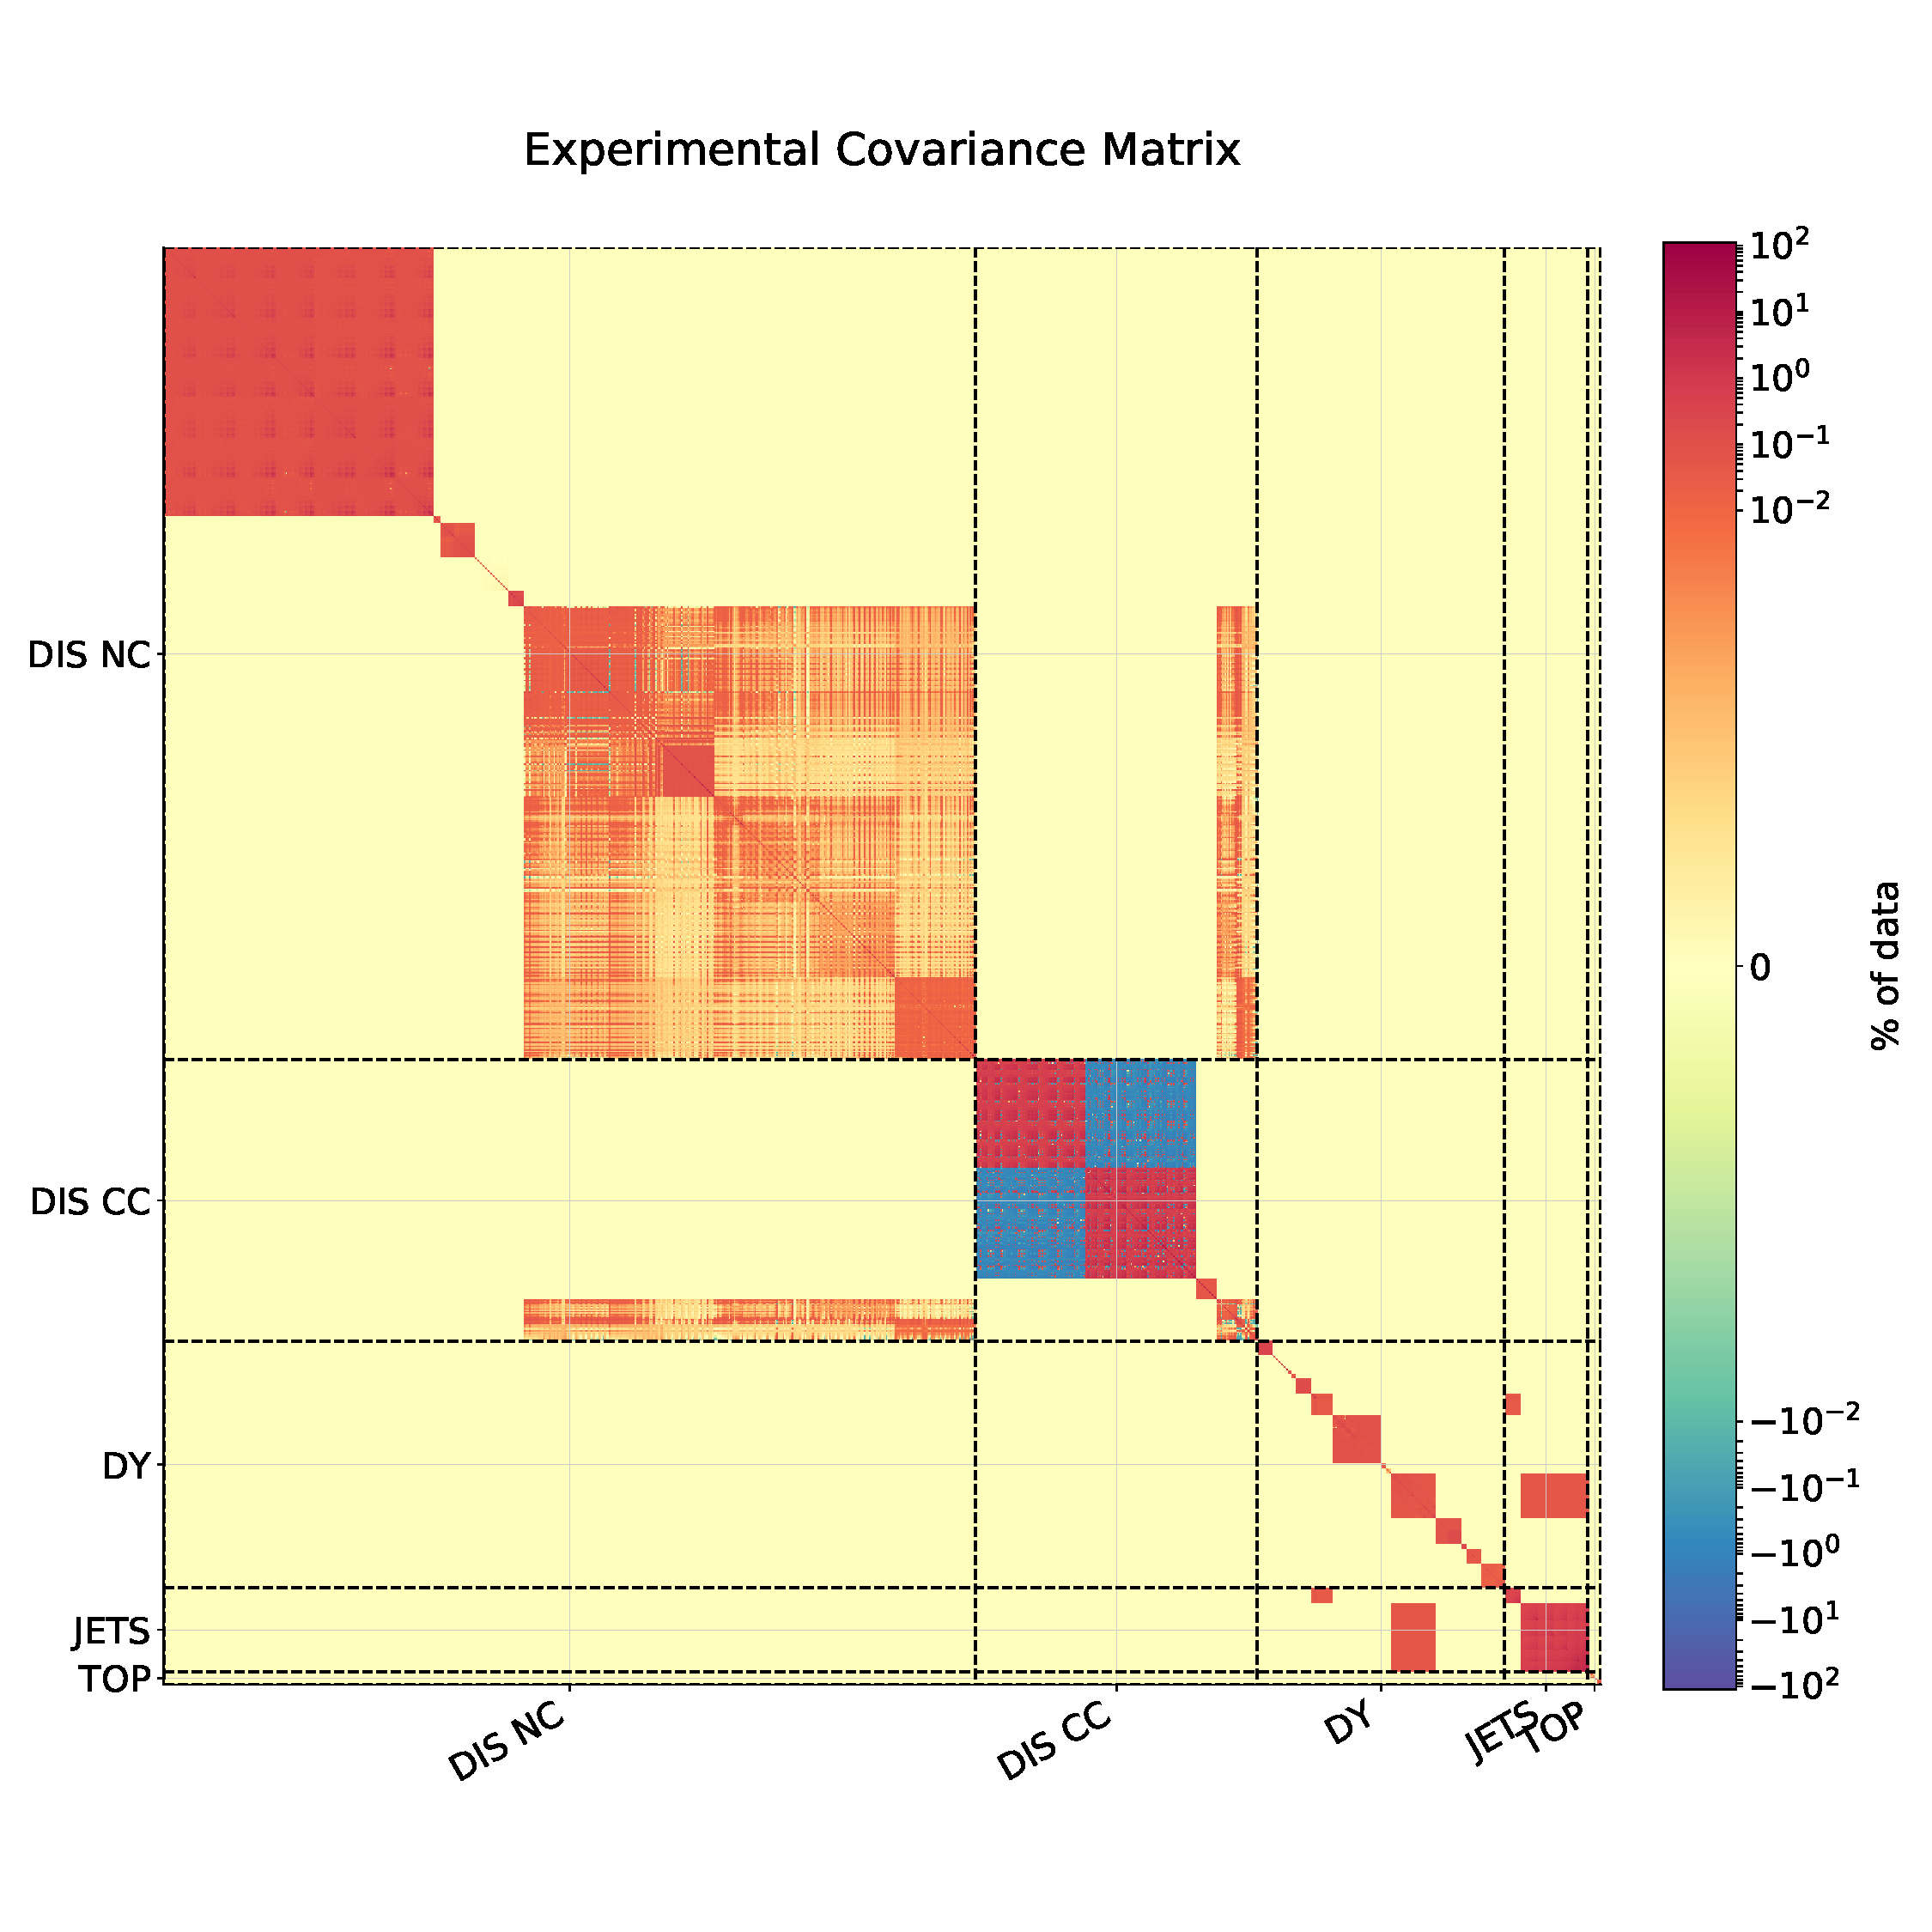
\includegraphics[width=0.49\hsize]{ch-pineline/exp_covmat}
	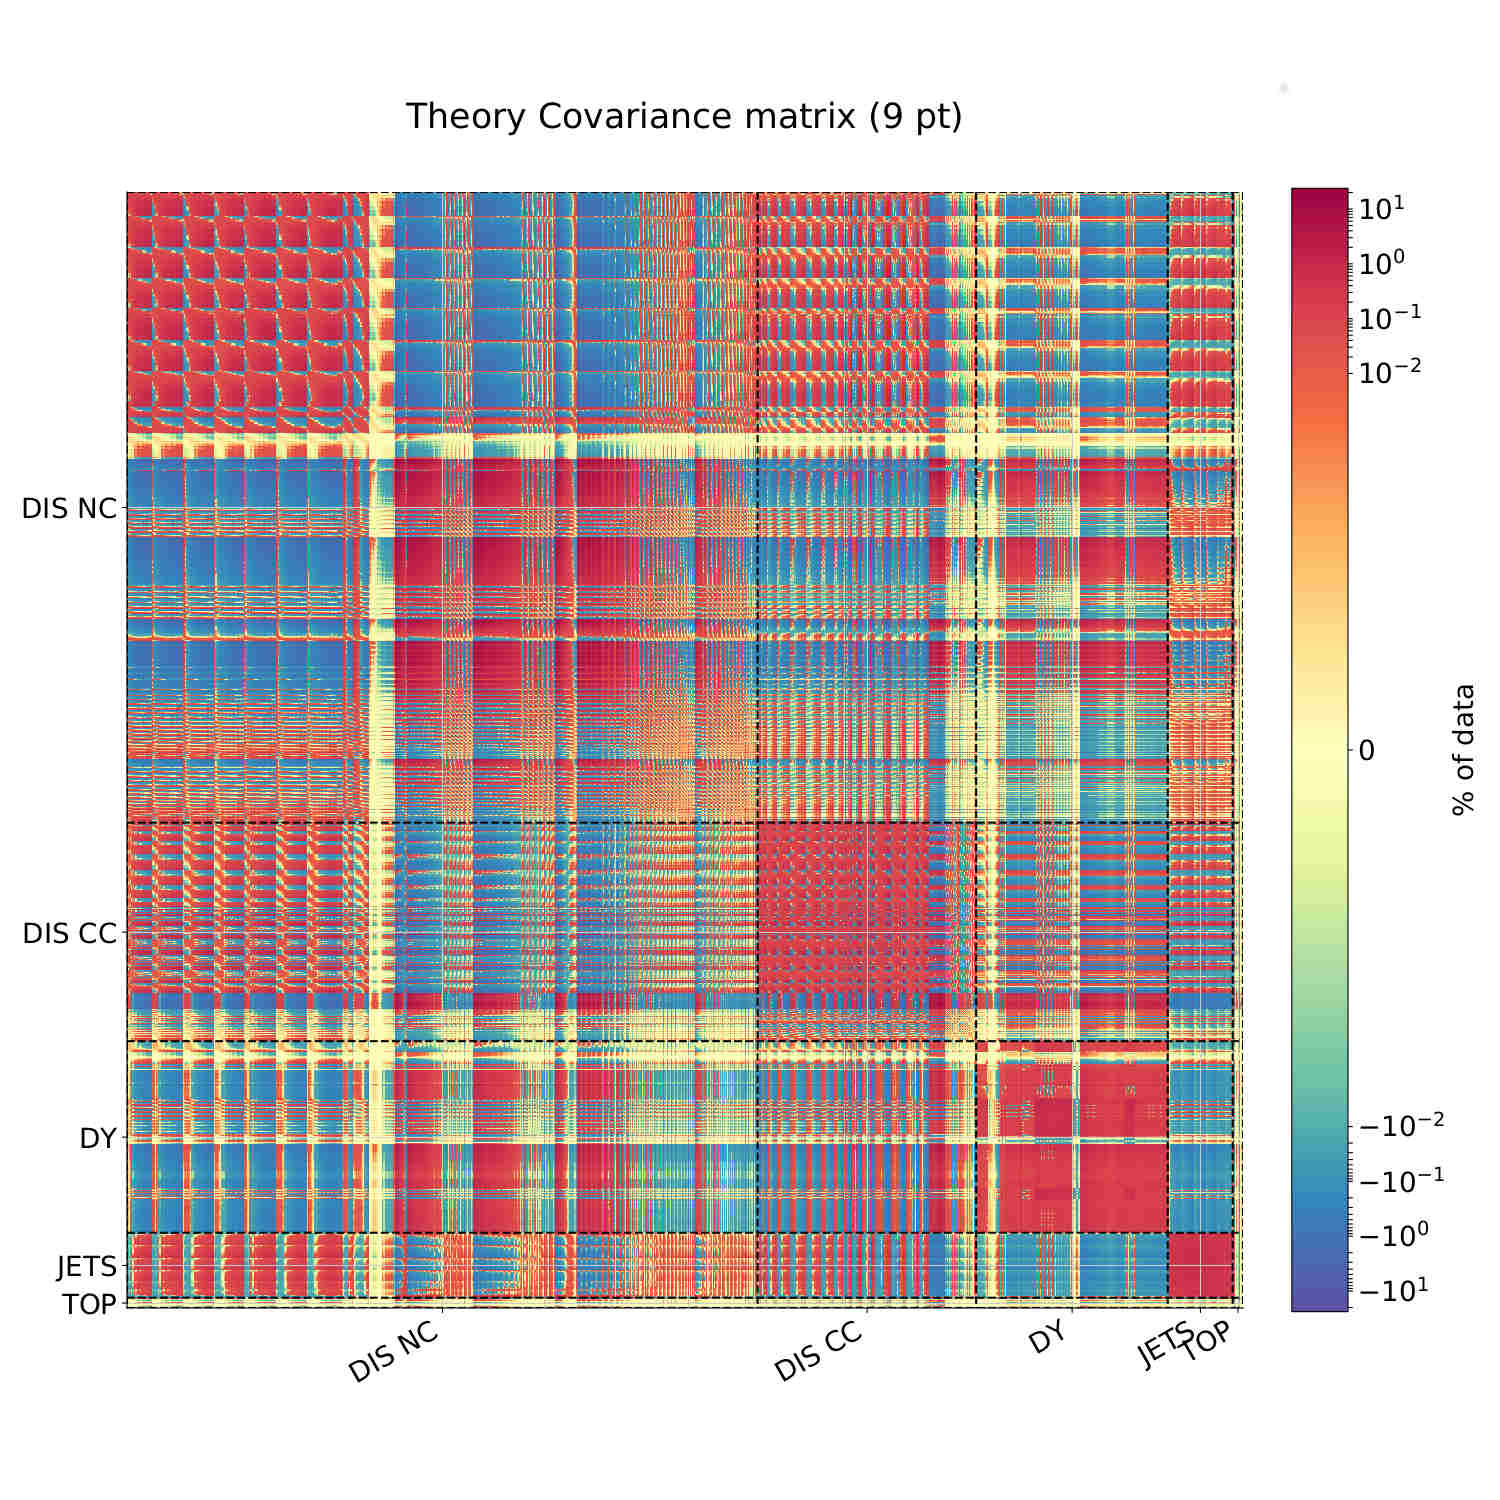
\includegraphics[width=0.49\hsize]{ch-pineline/th_covmat_9pt}
	\caption{
		Comparison between the experimental covariance matrix and the
		theoretical one, generated by the 9 point prescriptions, both
		normalized to central values.
	}
	\label{fig:pine/covmats}
\end{figure}

\begin{figure}
	\centering
	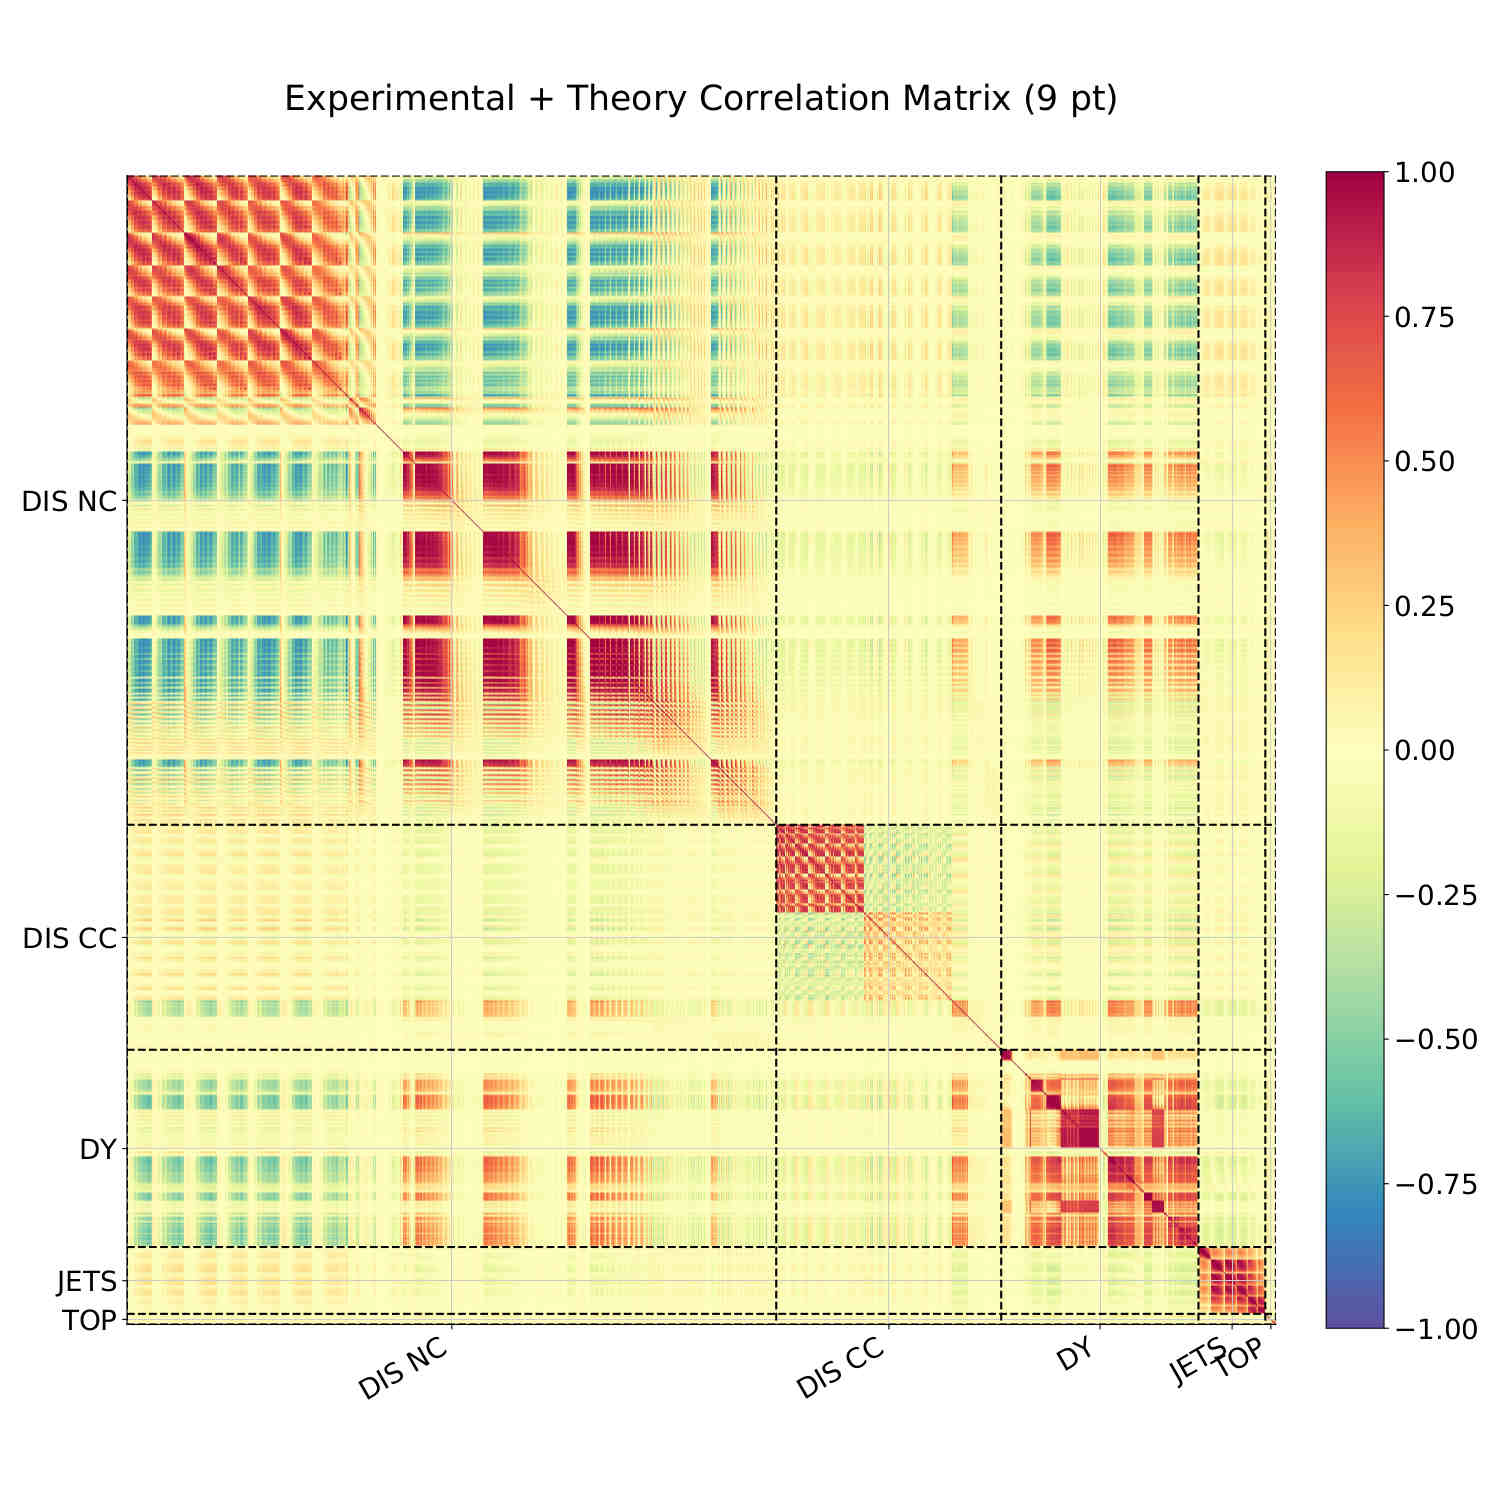
\includegraphics[width=0.7\hsize]{ch-pineline/expth_corrmat_9pt}
	\caption{
		Combined covariance matrix (experimental plus theoretical), the actual
		one used in the \nnpdfr[3.1th+]{3.1th} fit.
	}
	\label{fig:pine/combined-covmat}
\end{figure}

\begin{figure}
	\centering
	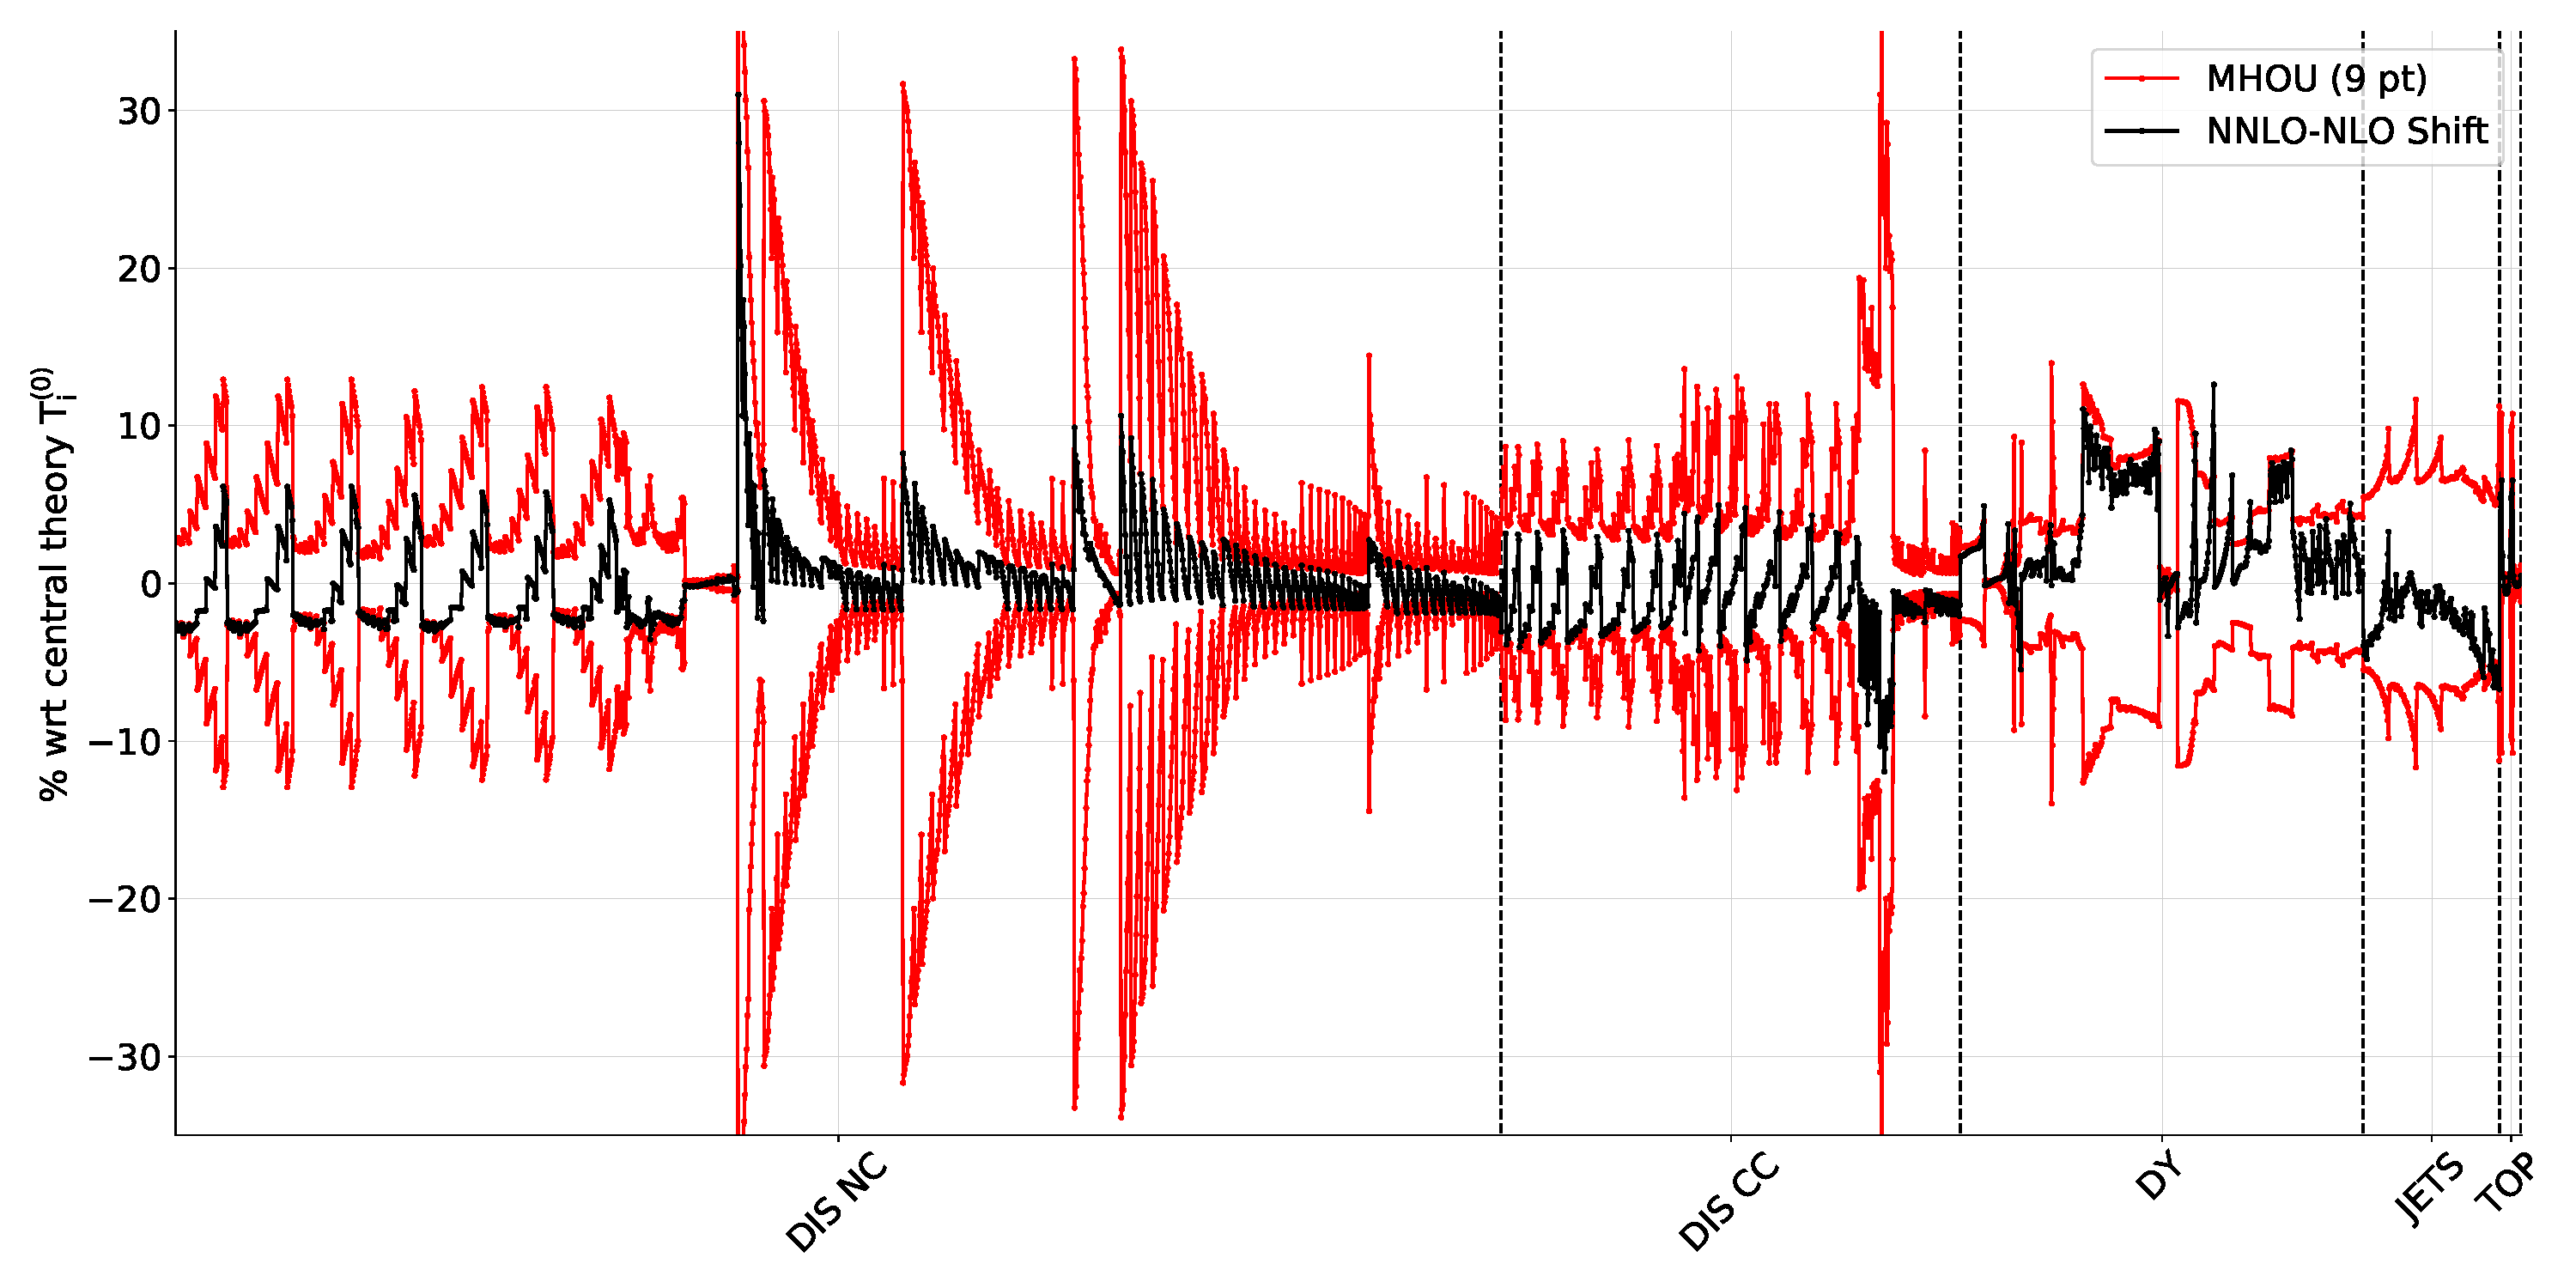
\includegraphics[width=\hsize]{ch-pineline/shift_diag_cov_comparison_9pt_global}
	\caption{
		The diagonal uncertainties $\sigma_i$ (red) symmetrized about zero,
		compared to the shift $\delta_i$ for each data-point (black).
		Values are shown as percentage of the central theory prediction
	}
	\label{fig:pine/scvar-shifts}
\end{figure}

\begin{figure}
	\centering
	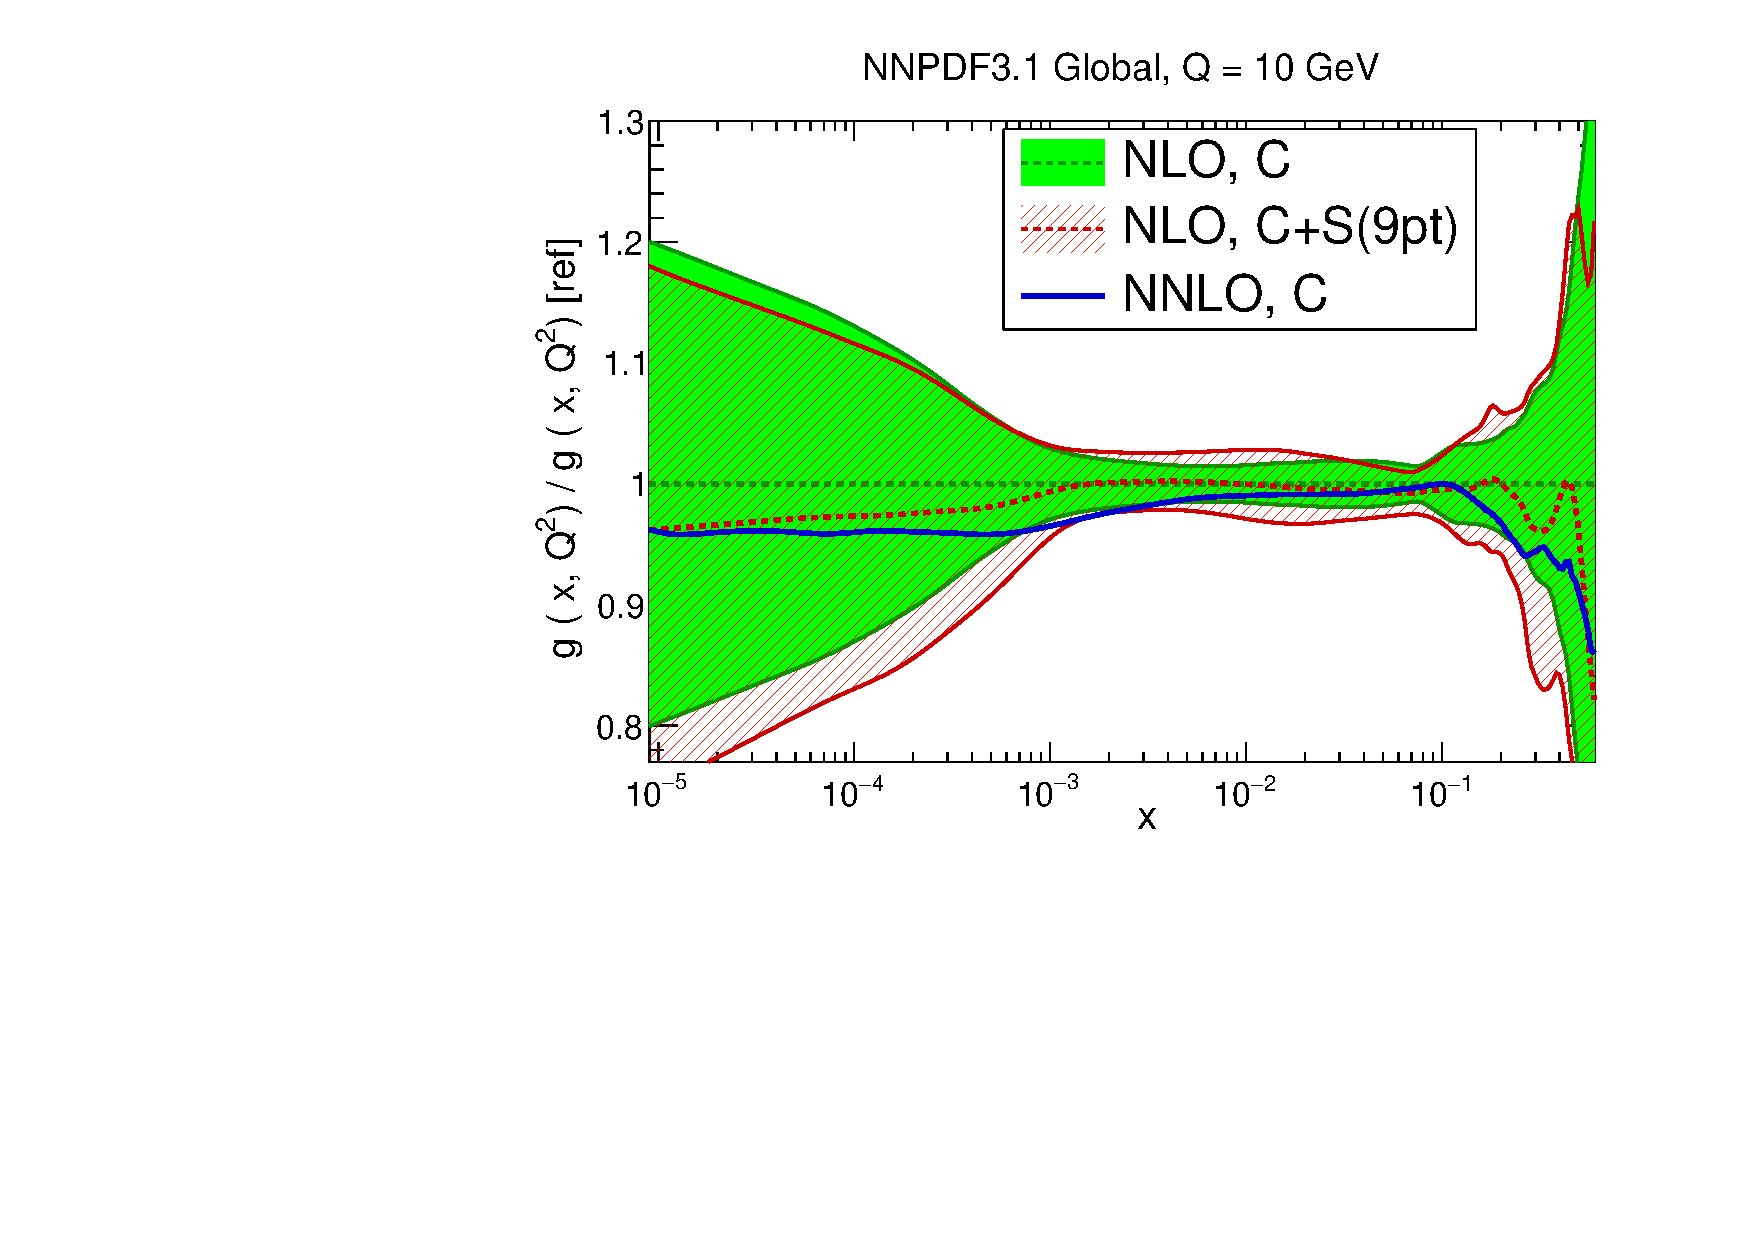
\includegraphics[width=0.49\hsize]{ch-pineline/xg-Global-NLO-CovMatTH-EXP-vsTH}
	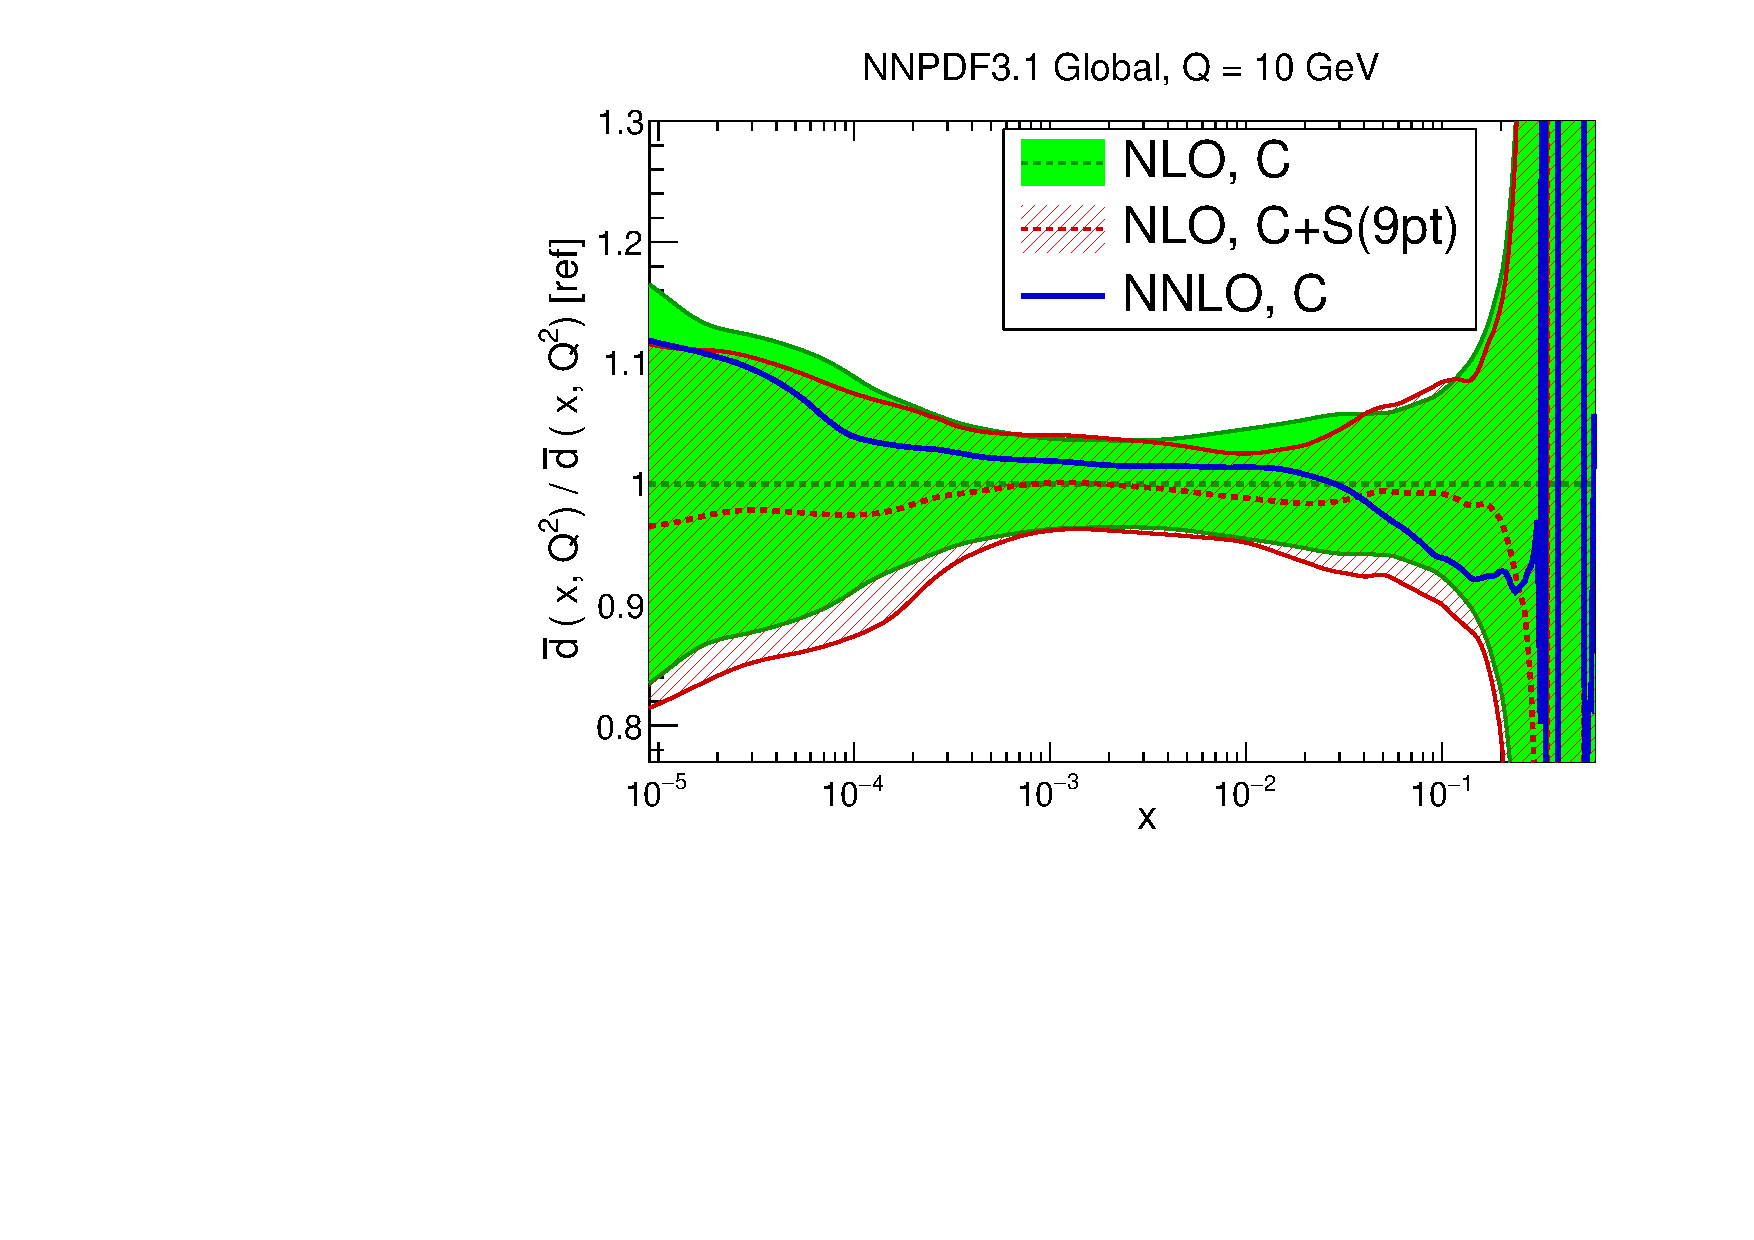
\includegraphics[width=0.49\hsize]{ch-pineline/xdbar-Global-NLO-CovMatTH-EXP-vsTH}
	\caption{
		\nnpdfr[3.1th+]{3.1th} \nlo sets, gluon and anti-down distributions at
		$\SI{10}{\giga\electronvolt}$, the first \pdf determination to include
		\mhou estimates in the fit.
	}
	\label{fig:pine/3.1th}
\end{figure}

\begin{figure}
	\centering
	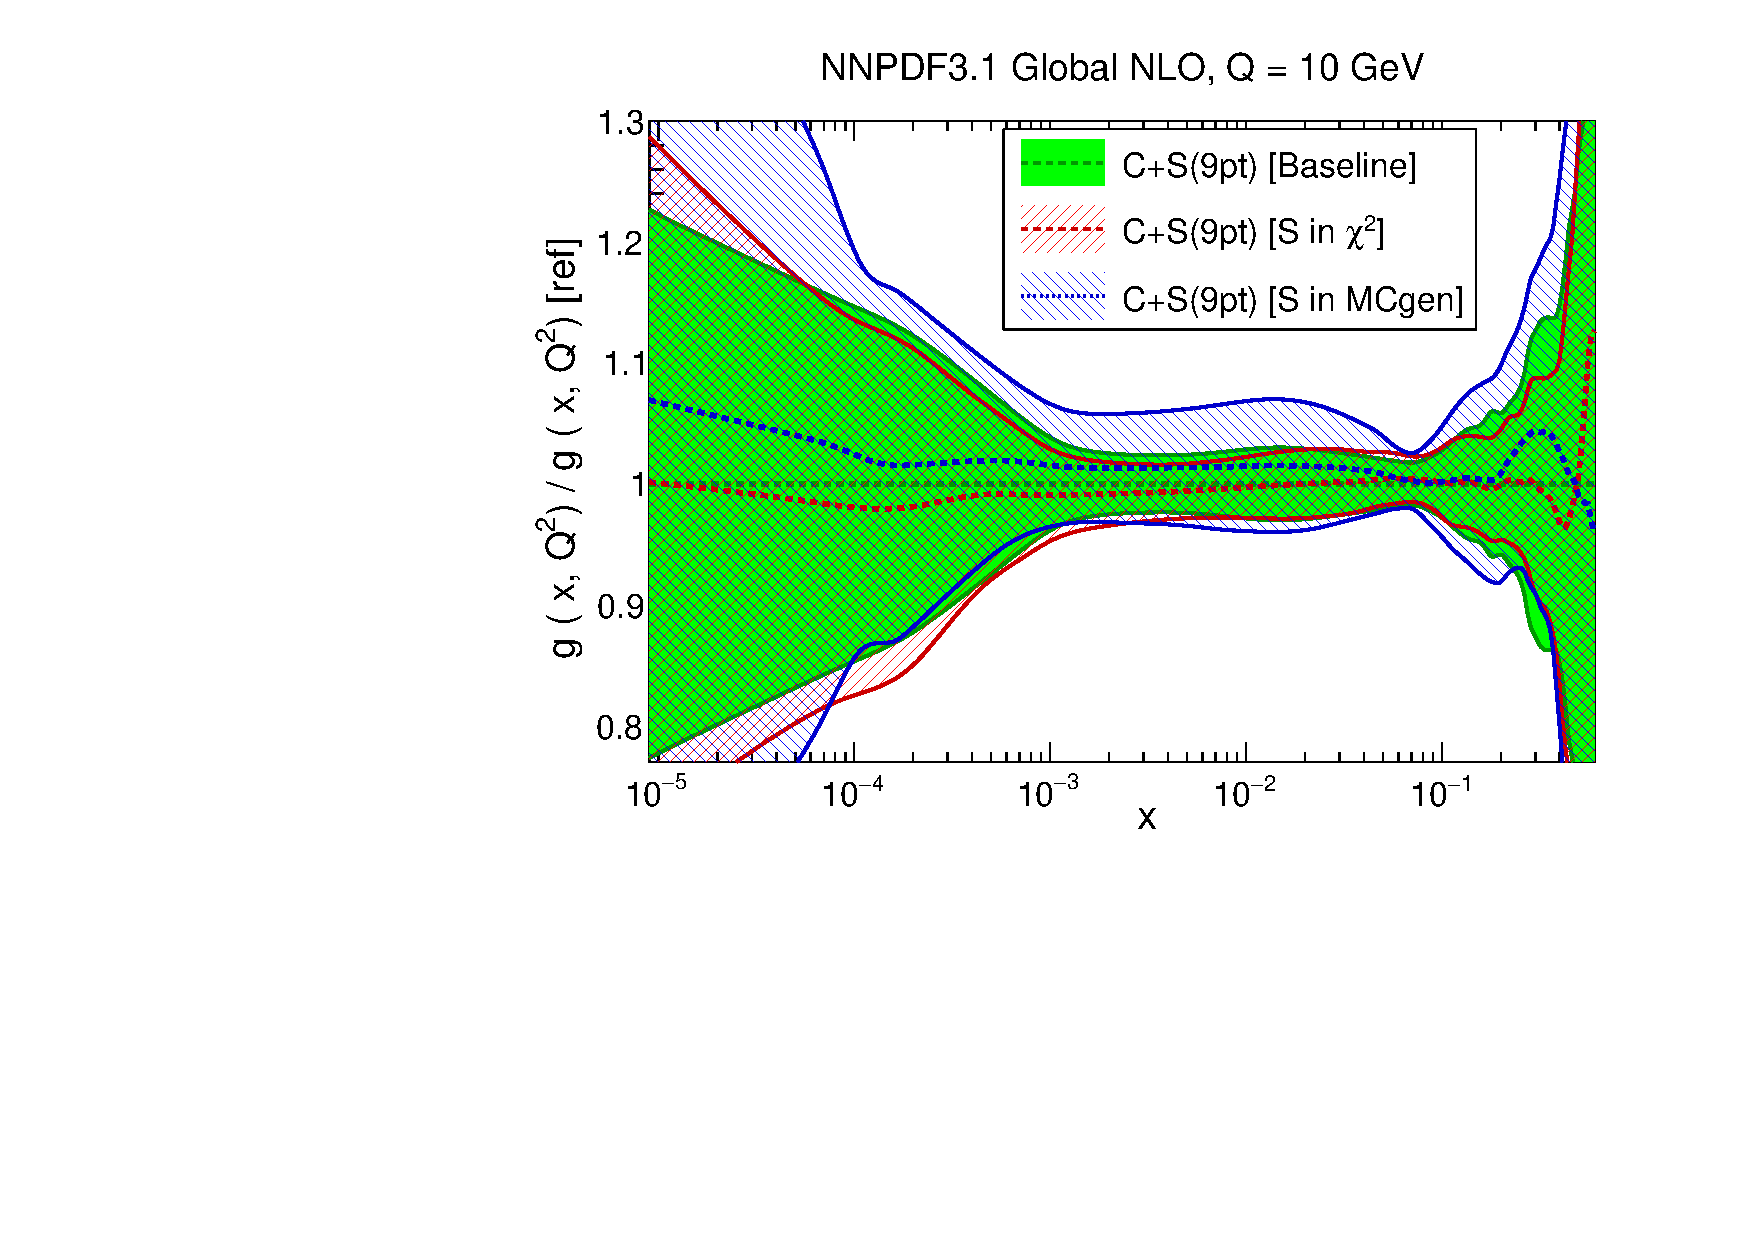
\includegraphics[width=0.49\hsize]{ch-pineline/xg-Global-NLO-CovMatTH-tests}
	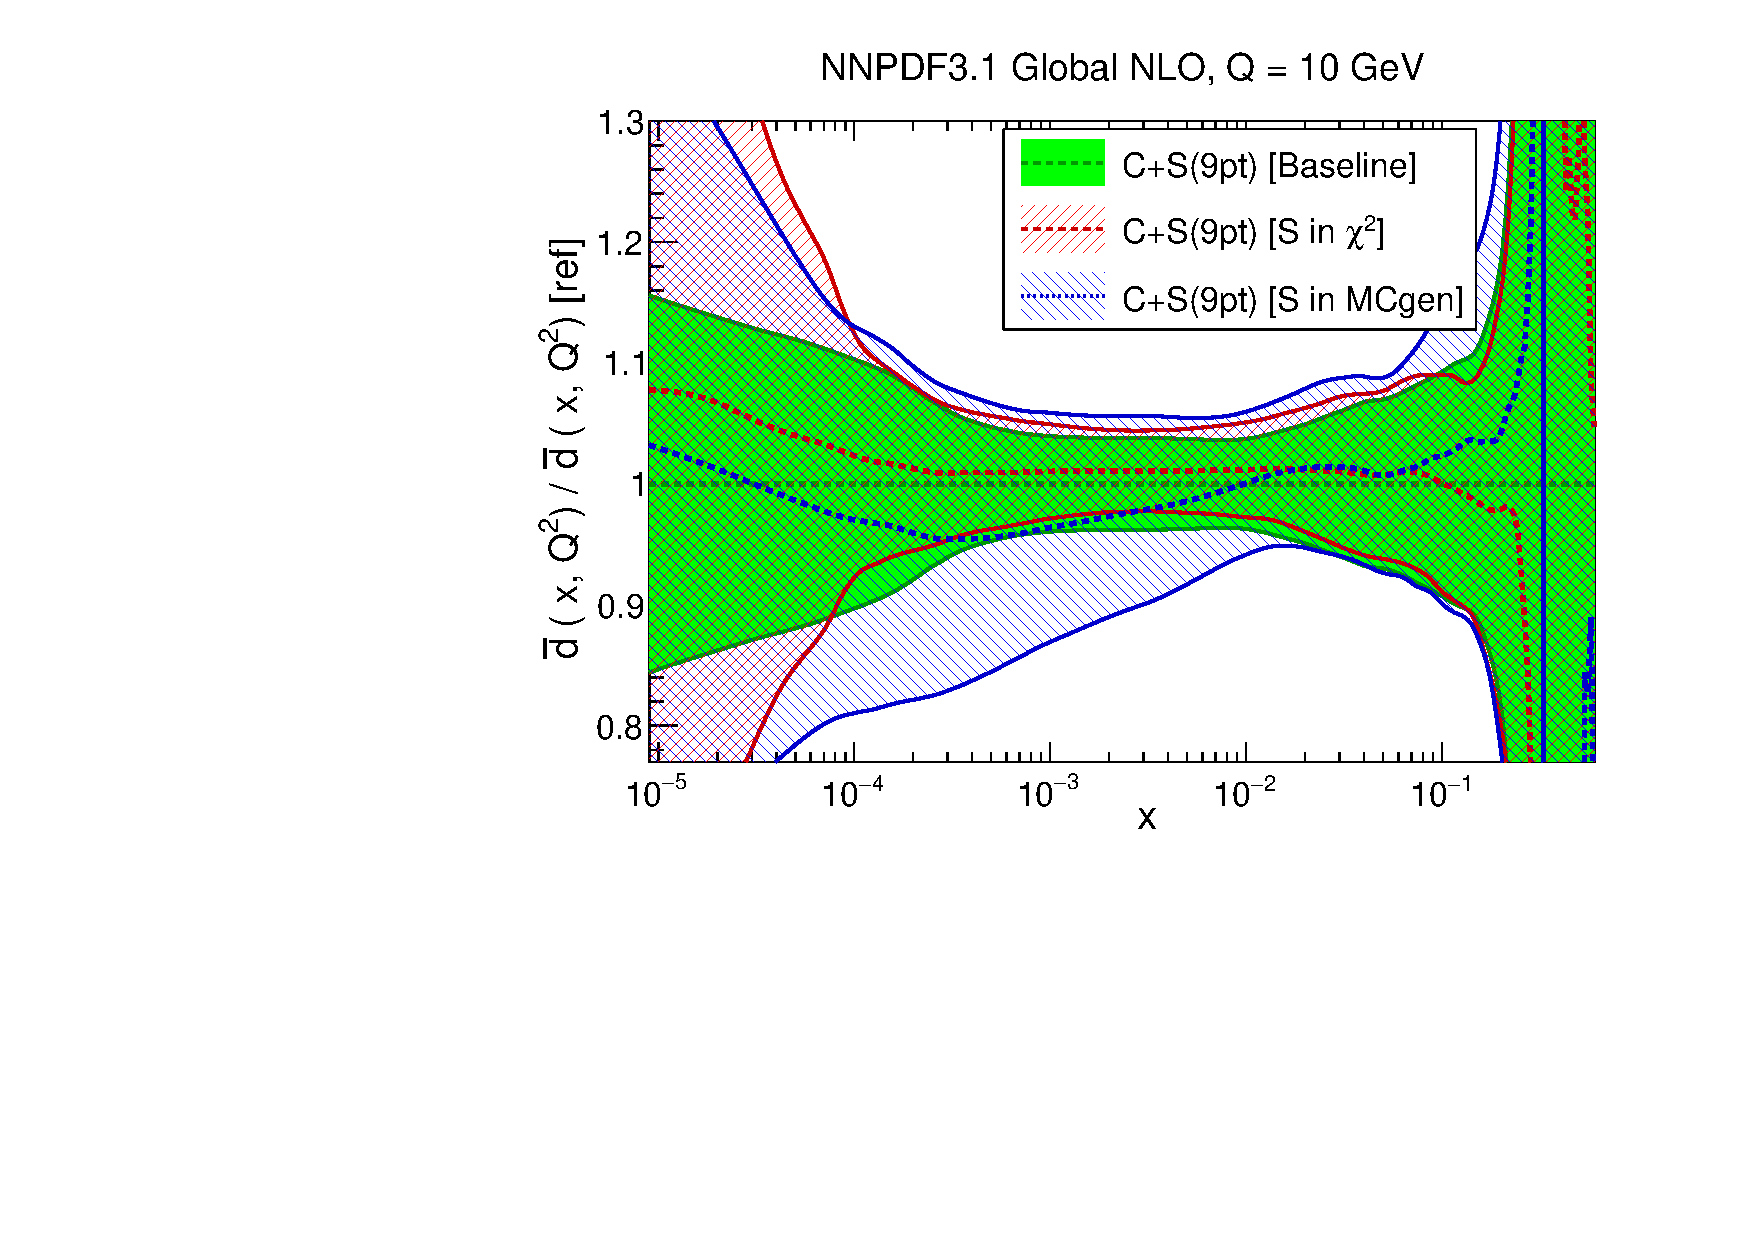
\includegraphics[width=0.49\hsize]{ch-pineline/xdbar-Global-NLO-CovMatTH-tests}
	\caption{
		Gluon and anti-down distributions comparison, in which it is shown the
		effect of using the theory covariance matrix in the $\chi^2$ or in the
		pseudo-data generation only.
	}
	\label{fig:pine/3.1th-tests}
\end{figure}


\vspace*{20pt}
\noindent
\rule{\hsize}{1pt}

\begin{itemize}
	\item brief history of MHOU in PDF fitting (cite NNPDF3.1th)
	\item theory covmat recap (take theory covmat plots from the paper)
	\item scheme B and fact scale in evolution
\end{itemize}


\vspace*{20pt}
\noindent
\rule{\hsize}{1pt}

\begin{itemize}
	\item brief history of MHOU in PDF fitting (cite NNPDF3.1th)
	\item theory covmat recap (take theory covmat plots from the paper)
	\item scheme B and fact scale in evolution
\end{itemize}

\section{New developments}
\label{sec:mhou/new}
% !TeX root = ../../../main.tex

The investigation in \cite{NNPDF:2019ubu} stopped at \nlo, because of various
technical limitations, and the lack of a proper benchmark to assess the
reliability of available implementations.
%
An \nnlo fit based on the theory covariance matrix formalism is still missing,
and this specific target will be achieved with the tools offered by the new
theory pineline (cf.\ \cref{ch:pine}).

A first update regards the actual implementation of scheme B, introduced in
\cref{sec:mhou/pdf}.
Indeed, scale variations in scheme A-like fashion has been the first and
default way they appeared in the evolution programs, starting with programs
like \pegasus.
In order to apply them, the \pdf anomalous dimensions have to be evaluated at a
scale shifted from the usual one, and a few extra terms appears.
%
But, being implemented at the anomalous dimensions level, these contributions
are resummed by the solution of the differential equations, and essentially
exponentiated (the solution of a linear differential equation is a path ordered
exponential of the associated kernel).
%
But this is not the contribution required by scheme B, and violates the scheme
C equivalence.
To get the expanded result, an extra piece has to be multiplied to the evolved
\pdf, so after solving the differential equation.
%
For this reason, \eko ships both the kind of factorization scale variations
(the only scale variations on the evolution side), dubbed
\textit{exponentiated} and \textit{expanded}, and the user can choose an actual
solution conformal to the scheme B prescriptions.
%
Since \eko does not produce evolved \pdfs, but evolution operators, the extra
piece appearing in the expanded case is also implemented at the anomalous
dimensions level, Mellin inverted, and included as an extra factor in the final
operator returned as output (i.e.\ it is not returned individually).

Another delicate point is the role of the strong coupling $\alpha_s$ in the
computation of factorization scale variations.
Indeed $\alpha_s$ appears in two places: as the parameter of the perturbative
series, evaluated at the scale of the process, and in the solution of \dglap
equations.
%
Indeed, the running coupling $\alpha_s(Q^2)$ is a monotonically decreasing
function of the scale, and contains the only scale dependence in the anomalous
dimensions.
Therefore, it is convenient to change variable, and solve \dglap as function of
$\alpha_s$, instead of the factorization scale.
%
This usage might suggest a relation between the strong coupling and the
factorization scale, and then the value used should be affected by the
related variations.
Instead, this is only used as a monotonic function, so for its mathematical
properties and the role in the equation (stemming from anomalous dimensions
perturbative expansion), and there is no implication about a physical relation.
%
Essentially, $\alpha_s$ value is only sensitive to renormalization scale
variations, that does not affect evolution at all, but it is used there as a
function of factorization scale.
This usage led to a clash in the options used, and a slightly wrong result when
both variations were applied, and it has been fixed in the current pineline.

Moreover, both renormalization scales variations (always coming from the
partonic cross-sections) and full scheme C (i.e.\ including also factorization)
can also be accomplished without requiring any information about scale
variations from the generators used.
The structure of the scale variations contributions consists substantially in
scale ratios logarithms multiplying lower order cross-sections, and the
coefficients of the perturbative expansion of the beta function of the strong
coupling $\beta(\alpha_s)$ (renormalization) or the splitting
functions/anomalous dimensions $P(x, \alpha_s)$.
%
If the interpolation grid is stored separately by order, it is then possible to
reconstruct the missing dependence on the two scales, as described in section
2.3 of \cite{Carli:2010rw}.
%
However, the reconstruction of factorization scale dependence requires
convolutions with increasingly complex distributions (with the perturbative
order), i.e.\ more or less the same complexity of a \dis coefficient functions
integration, as it is performed by \yadism.
But they are also the universal ingredient.
%
So, we decided for a mixed approach: keep using scheme B there is no need for
factorization scale dependence to be stored in or computed from the grids (the
original reason to advocate for this scheme, over the C option), but we can
reconstruct the renormalization scale dependence, just relying on a fixed set
of numerical coefficients ($\beta$ function expansion), completely removing the
need to obtain scale variations from external providers.

Finally, using both the ingredients provided by the \eko and \yadism libraries,
we benchmarked our implementations of scale variations with some analytical
results, based on the expressions for some specific \dis contributions, order
by order and for specific partonic channels.
%
This already allowed us to resolve the small differences between scheme B and
C, and confirm that they are always higher order contributions, even though the
difference in the actual values is only negligible in most of the cases, but
not all of them, becoming sizeable in specific kinematic corners (from few
percent up to $\sim 20\%$).
%
A few channels are still missing at \nnlo, and the full benchmark will be
presented in a separate publication about the \mhou treatment with the new
pineline, possibly the release of the first \nnlo \nnpdf set accounting for
\mhou.


\vspace*{20pt}
\noindent
\rule{\hsize}{1pt}

\begin{itemize}
	\item actual scheme B implementation in \eko - as opposed to exponentiated
		in \apfel, i.e.\ same as \pegasus but used for B: not an issue, but it
		differs more from C, common in \mc generators
	\item what we updated wrt to NNPDF3.1th ($\alpha_s$ function vs value, and
		how ren scale vars where entering DGLAP)
	\item what is missing for a new theory covmat
	\item generate ren scale dependency in grids
\end{itemize}

\section{Scale variations -- point prescriptions}
\label{sec:mhou/prescriptions}
% !TeX root = ../../../main.tex

We describe the derivation of suitable point prescriptions, that can be
used in the construction of a positive semi-definite theory covariance
matrix.
It turns out that two classes of prescriptions are possible, both requiring
milder or stronger generalization of equations in \cite{NNPDF:2019ubu}.
The actual result claimed in the paper can be obtained within the broader
generalization, ensuring the positive semi-definiteness of the covariance
matrix computed with that class of prescriptions.

\subsection{Introduction}
\label{sec:intro}
% !TeX root = ../../../main.tex

The first fundamental application of the integrated pineline will actually the
inclusion of \acrfull{mhou} at \nnlo in the \nnpdfr{4.0} fit.

\pdfs are non-perturbative objects, so it may seem counter-intuitive that their
accuracy depends on perturbative series truncation.
%
This is a direct consequence of extracting them from high energy collisions
data: they are completely determined by physics that happens in the
perturbative regime, and the map discussed at the beginning of this chapter
(the one that connects data to \pdfs) is completely determined by \pqft
calculations.
%
So, the origin of the perturbative order of \pdf sets is exactly determined by
the theory predictions used during the extraction: a \nnlo set is a \pdf set
that has been fitted using theory predictions at \nnlo.
%
A \pdf set directly computed with non-perturbative methods would have no
perturbative order associated, even when used in a perturbative calculation
\footnote{
	From that point of view would be an \textit{all-order} object, even though
	it might be subject to other kinds of approximations.
}\footnote{
	Also consider that \dglap evolution is perturbative, so, once evolved, it
	acquires again a dependency on the perturbative truncation.
}.

The perturbative series enters in the \pdf in two different places: the
partonic cross section calculations (those encoded in \textit{grids}) and the
\dglap evolution\footnote{
	That technically is used twice: during the fit, to bridge data with the
	boundary condition candidate, and to evolve the final boundary condition to
	all scales.
	But considering the \pdf a function of two variables ($z$ and $\mu_F^2$)
	consistently, the abstract evolution flow used is a single one.
}.
%
In principle, these are two different perturbative orders, thus there is not a
single truncation, but two of them, and they can happen at two different
orders.
%
Still, the two objects are not completely decoupled: \dglap evolution arise
from collinear divergences, subtracted by the chosen factorization scheme.
These collinear logarithms appear as well in the partonic cross sections, so it
is important to properly account for them, avoiding double counting.
%
The whole picture of collinear subtractions is deeply connected to treatment of
quark masses, better discussed in \cref{ch:dis}, since a finite value of the
mass regulates the collinear divergence on its own.
%
Therefore, the double perturbative order already appears in the partonic cross
sections calculations, where the \fns chosen can account for light and heavy
quarks at two distinct orders (cf. \cite{Forte:2010ta}, in particular the
FONLL-B scheme).


\subsection{Derivation}
\label{sec:deriv}
Once all the elements in \cref{eq:shifts,eq:thcovmat} are spelled out, we have a clear
recipe on how to compute the covariance matrix $S_{ij}$.

For this reason, we are going to exploit all the properties that are required
or desirable (advantageous), in order to limit the available degrees of
freedom: anything left, it has to be regarded as being part of the
\textit{prescription}.

The current degrees of freedom are:

\begin{enumerate}
    \item the choice of the $p + 1$ dimensional space $\mathcal{V}_{ij}$ of all
        the accounted variations ($p$ renormalization scales, $1$ factorization
        scale)
    \item the choice of normalization coefficients $c_i(\vec{\kappa}) \in \R$
        \footnote{
            Not all values of $\R$ make sense, but there is quite a wide range
            of interesting variations: $\N$ for repeated points, or $\Q^+$ for
            normalizations (possibly coming from repeated points), or $0$ for
            masking.
            At this level, we are just not excluding anything that has no
            special reason to be excluded.
        }
    \item the choice of the default value $\vec{\kappa}_0$
\end{enumerate}

The last element is trivial: it's going to be part of the prescription, but in
the following we will always write $\vec{\kappa}_0 = \vec{0}$ for definiteness
(it's simple to replace this in the final result with $\vec{\kappa}_0$ in any
case).

\paragraph{Extra scales} We know that the predictions for each data point only
depend on two scales: the common factorization scale, and the related
renormalization scale, but not the others.
For this reason, it makes no sense to pick the normalization for point $i$
dependent on the other scales, since it would introduce a dependency of the
shifts on those scales that was not present in the unnormalized shifts.
Thus:

\begin{equation}
    \label{eq:2dim-norm}
    c_i(\vec{\kappa}) \equiv c_i(\kappa_F, \kappa_{R,i})
\end{equation}

\paragraph{Per-pair space} Next, we claim that the space $\mathcal{V}_{ij}$ can
not actually depend on the element $ij$ of the covariance matrix been
constructed. Indeed this stems directly for the necessity to prove
\cref{eq:pos} that is done in the following way:

\begin{align}
    \sum_{i,j} v_i S_{ij} v_j &= \sum_{i,j} \sum_{\vec{\kappa} \in \mathcal{V}_{ij}} v_i \Delta_i(\vec{\kappa})\Delta_j(\vec{\kappa}) v_j  =\\
        &= \sum_{\vec{\kappa} \in \mathcal{V}} \sum_{i,j} v_i \Delta_i(\vec{\kappa})\Delta_j(\vec{\kappa}) v_j =\\
        &= \sum_{\vec{\kappa} \in \mathcal{V}} \left(\sum_{i} v_i \Delta_i(\vec{\kappa})\right)^2 > 0
\end{align}

If the space $\mathcal{V}$ were actually dependent on $ij$, it would have not
been possible to swap the two sums in the second step.

\paragraph{Space choice} On the other hand, it is desirable to define the
prescription only on the space of relevant scales for the given point $ij$.
This means the factorization scale $\kappa_F$ and

\begin{description}
    \item[off-diagonal] two renormalization scales $\kappa_{R,i}$ and
        $\kappa_{R,j}$, or
    \item[diagonal] even a single one, if the two points are related to the
        same process, i.e. 
        \begin{equation*}
            \kappa_{R,i} = \kappa_{R,j}
        \end{equation*}
\end{description} 

We would like our expressions not to depend on the number of scales present,
and only account for the scale relevant for the pair $ij$ being considered.
The easiest choice is to pick the space $\mathcal{V}$ to be fully factorized in
the various dimensions of $\vec{\kappa}$. This means that it can be written as
\begin{equation}
\mathcal{V} = \prod_{i = 1}^{p+1} v_{i},
\end{equation}
with $v_{i}$ the one-dimensional space representing the variation of the single
scale labeled with $i$. 
\newline

But this is not the only choice available, it is just the simplest.
There is only one more option that guarantees the independence of the
projection on the pair $ij$, i.e. factorize the space for each possible value
of $\kappa_F$.
This option will be explored in \cref{sec:mhou/prescr/slices}.
\newline

In the case of a fully factorized space, the complex choice of the space is
reduced on $p + 1$ choices for one dimensional spaces.
But if there is no reason to distinguish processes at this level, it is
reasonable to pick the same space for each renormalization scale.

In practice, the basic one dimensional space will be always the same\footnote{
    The one spelled out is only an option, any other space would work equally
    well.
}:
\begin{equation}
    \label{eq:1dim-space}
    v = \{-\log(2), 0, \log(2)\} \equiv \{-, 0, +\}
\end{equation}
and the overall space will be just the product:
\begin{equation}
    \mathcal{V} = v^{p + 1}
\end{equation}

\paragraph{Normalization} At this point, all the arbitrariness left for the
prescription is encoded in the normalization coefficients.
With our simple choice of the space there is no reason to choose complex
coefficients, thus we will define the following prescriptions:

\begin{equation}
\label{eq:norm_coeff}
    c_i(\vec{\kappa}) = 
    \begin{cases}
        1 / \sqrt{N_m}     \qquad &\kappa \in \mathcal{V}^i_m\\
        0                  \qquad &\text{else}
    \end{cases}
\end{equation}

The spaces $\mathcal{V}_m^i$ now defines our point prescription, together with
the overall normalization $N_m$, since the $c_{i}(\vec{\kappa})$ are acting as \textit{masks} on the points $\vec{\kappa}$ not belonging to the space.
For the former we'll choose:
\begin{equation}
    \mathcal{V}_m^i = v_m^i \times \{-, 0, +\}^{p-1}
\end{equation}
where the two dimensional spaces $v_m^i$ are always the same space $v_m$, but
for the scales $(\kappa_F, \kappa_{R,i})$, while the other scales are free to
assume any possible value.

For the normalizations instead, there is no strict nor reasonable way to fix it
completely, but it is possible to fix the scaling in the case of a space
$v_m$ and $v$ with an hypothetically large number of point: since we don't want
the normalization of the theory covariance matrix to depend on the number of
points being in the prescription, we'll choose
\begin{equation}
    \label{eq:N-norm}
    N_m \propto \abs{v_m} \cdot \abs{v} = m \cdot 3^{p-1}
\end{equation}


\subsection{Alternative space: $\kappa_F$ slices}
\label{sec:slices}
In \cref{sec:mhou/prescr/deriv} we made a set choices for the degrees of
arbitrariness exposed at the beginning.
All of them were yield by a strict requirement (needed to obtain a property,
like $S_{ij} \ge 0$) or by a reasonable request (e.g.\ not adding further
dependencies with normalizations, which led to \cref{eq:mhou/prescr/2dim-norm}).
Only in one single case we made an assumption based on an unneeded simplicity:
the choice of the space as fully factorized.

This choice is sensible for the renormalization scales: why should the space
look different seen from the perspective of different processes? Why different
processes should be correlated by the space?
On the other hand, it is completely arbitrary for the factorization scale.
Since factorization scale $\kappa_F$ is treated separately from renormalization
scales $\kappa_{R,i}$, no surprise if even the space symmetry somehow is broken
on $\kappa_F$\footnote{
    For the $\kappa_{R,i}$, choosing them factorized and uniform as argued, a
    permutation invariance is present, and makes sense.
    No reason to extend it to $\kappa_F$.
}.

Thus, we can have a different factorized space for each different value of $\kappa_F$:
\begin{align}
    \label{eq:mhou/prescr/sliced-space}
    \mathcal{V} &= \bigsqcup_{\kappa_F \in v_F} \mathcal{V}(\kappa_F)\\
    \label{eq:mhou/prescr/1f-factorized}
    \mathcal{V}(\kappa_F) &\equiv v(\kappa_F)^p
\end{align}
where $v_F$ is the space of possible values of $\kappa_F$ (usually it will be
just $v$ of \cref{eq:mhou/prescr/1dim-space}), and $v(\kappa_F)$ is instead the space of
renormalization scales related to that single value of the factorization scale.

In this case also the definition of the normalizations $c_i(\vec{\kappa})$
should change with respect to those defined in \cref{eq:mhou/prescr/norm_coeff} in order to
account for this, since the different spaces contain different numbers of
points.
We decide to normalize the elements such that once the full space is projected
over each of the two dimensional spaces $(\kappa_F, \kappa_{R,i})$, the
coefficients of the various shifts are equal to one, thus:
\begin{equation}
    \label{eq:mhou/prescr/sliced-norm}
    c_i(\vec{\kappa})^2 \propto \frac{1}{\sum_{\kappa_F'}v(\kappa_F')} \frac{\abs{v(\kappa_F)}}{\abs{\mathcal{V}(\kappa_F)}}
        = \frac{1}{m \cdot \abs{v(\kappa_F)}^{p-1}}
\end{equation}
since the scales projected are all renormalization scales but a single one,
that is the relevant one for the given $i$, and together with $\kappa_F$ make
the two dimensional space, whose volume is $\sum_{\kappa_F'}v(\kappa_F') = m$.


\subsection{Conclusions}
\label{sec:concl}
% !TeX root = ../../../../main.tex

Two classes of possible prescriptions are identified:

\begin{enumerate}
    \item full space, with some zero coefficients
    \item sliced space, with factorization scale dependent normalizations
\end{enumerate}

No one of the two is strictly allowed by Eqs.\ (4.1) and (4.2) of
\cite{NNPDF:2019ubu}, since both require the usage of non-trivial
normalizations $c_i(\vec{\kappa})$, while the only normalization allowed by
Eq.\ (4.2) is a global one for the whole matrix.

Moreover, Eqs.\ (4.1) and (4.2) itself does not coincide with the correct and
general \cref{eq:mhou/prescr/shifts,eq:mhou/prescr/thcovmat}, because Eq.\
(4.2) is already defined at the level of a subspace $V_m$ of the large space
$\mathcal{V}$, and while this are described in the following, no proof is given
of the compatibility of this subspaces as projections of the full one.

Finally, the notation used in \cite{NNPDF:2019ubu} is confusing, since Eq.\
(4.2) gives the impression that the first shift $\Delta_i$ and the second shift
$\Delta_j$ are potentially evaluated on different points, while the point has
to be always the same, simply the actual dependence of the shifts is on two
different scales.
We advocate for a more explicit and transparent syntax, at least while defining
the general landscape for prescriptions (while at the individual prescription
level a more concise syntax might even be useful, if properly introduced in
relation to the general one).


